% this document is part of the DoCrimes project.
% Copyright 2022 the authors

\documentclass[modern]{aastex631}
\usepackage[utf8]{inputenc}

% typesetting issues
\sloppy\sloppypar\raggedbottom\frenchspacing

% figure issues
\usepackage[framemethod=tikz]{mdframed}
\usetikzlibrary{shadows}
\definecolor{captiongray}{HTML}{555555}
\mdfsetup{%
  innertopmargin=2ex,
  innerbottommargin=1.8ex,
  linecolor=captiongray,
  linewidth=0.5pt,
  roundcorner=5pt,
  shadow=true,
  shadowcolor=black!05,
  shadowsize=4pt
}
\newlength{\figurewidth}
\setlength{\figurewidth}{0.75\textwidth}

% math definitions

% text definitions
\shortauthors{hogg and storey-fisher}
\shorttitle{testing isotropy and homogeneity}

\begin{document}

\title{%
Testing cosmic isotropy and homogeneity
with \textsl{Gaia} quasars}
\author{David W. Hogg}
\affil{Center for Cosmology and Particle Physics, New York University}
\affil{Max-Planck-Institut f\"ur Astronomie}
\affil{Flatiron Institute, a division of the Simons Foundation}

\author{Kate Storey-Fisher}
\affil{Center for Cosmology and Particle Physics, New York University}

\date{2022 August}

\begin{abstract}\noindent
All cosmological models in general relativity are built on the assumption of large-scale isotropy and homogeneity.
These assumptions are testable.
Tests of cosmic isotropy and homogeneity are also strong tests of the quality of data or catalogs and their calibration.
Test precision increases as observations cover more solid angle, become more sensitive to distant objects, and are made with more uniform data.
The ESA \textsl{Gaia} Mission is primarily concerned with stars in the Milky Way, but it also observes millions of quasars, all sky (modulo Galactic extinction), to redshifts of around $4.5$.
It has produced the largest-comoving-volume public quasar catalog to date.
Here we use a carefully curated subsample of ZZZ \textsl{Gaia} quasars to show that the angular distribution, redshift distribution as a function of sky position, amplitude of clustering as a function of sky position, and counts of pairs as a function of separation (fractal dimension), are all consistent with large-scale isotropy and homogeneity at the precision possible given the size of the catalog and the amplitude of the large-scale structure.
Roughly speaking, the results can be summarized by saying that they show the Universe to be isotropic to better than XXX percent and homogeneous to better than YYY percent.
There is no sign of any North--South power asymmetry.
The isotropy results can also be interpreted as a strong test of the spectrophotometric uniformity of the \textsl{Gaia} Catalog.
\end{abstract}

\keywords{%
calibration
---
catalogs
---
cosmic~isotropy
---
cosmological~principle
---
cosmology
---
large-scale~structure~of~the~Universe
---
quasars
}

\section{Introduction}

Hello World!

\section{Data}

\begin{figure}[t!]
  \begin{mdframed}
  \color{captiongray}
  \begin{center}
    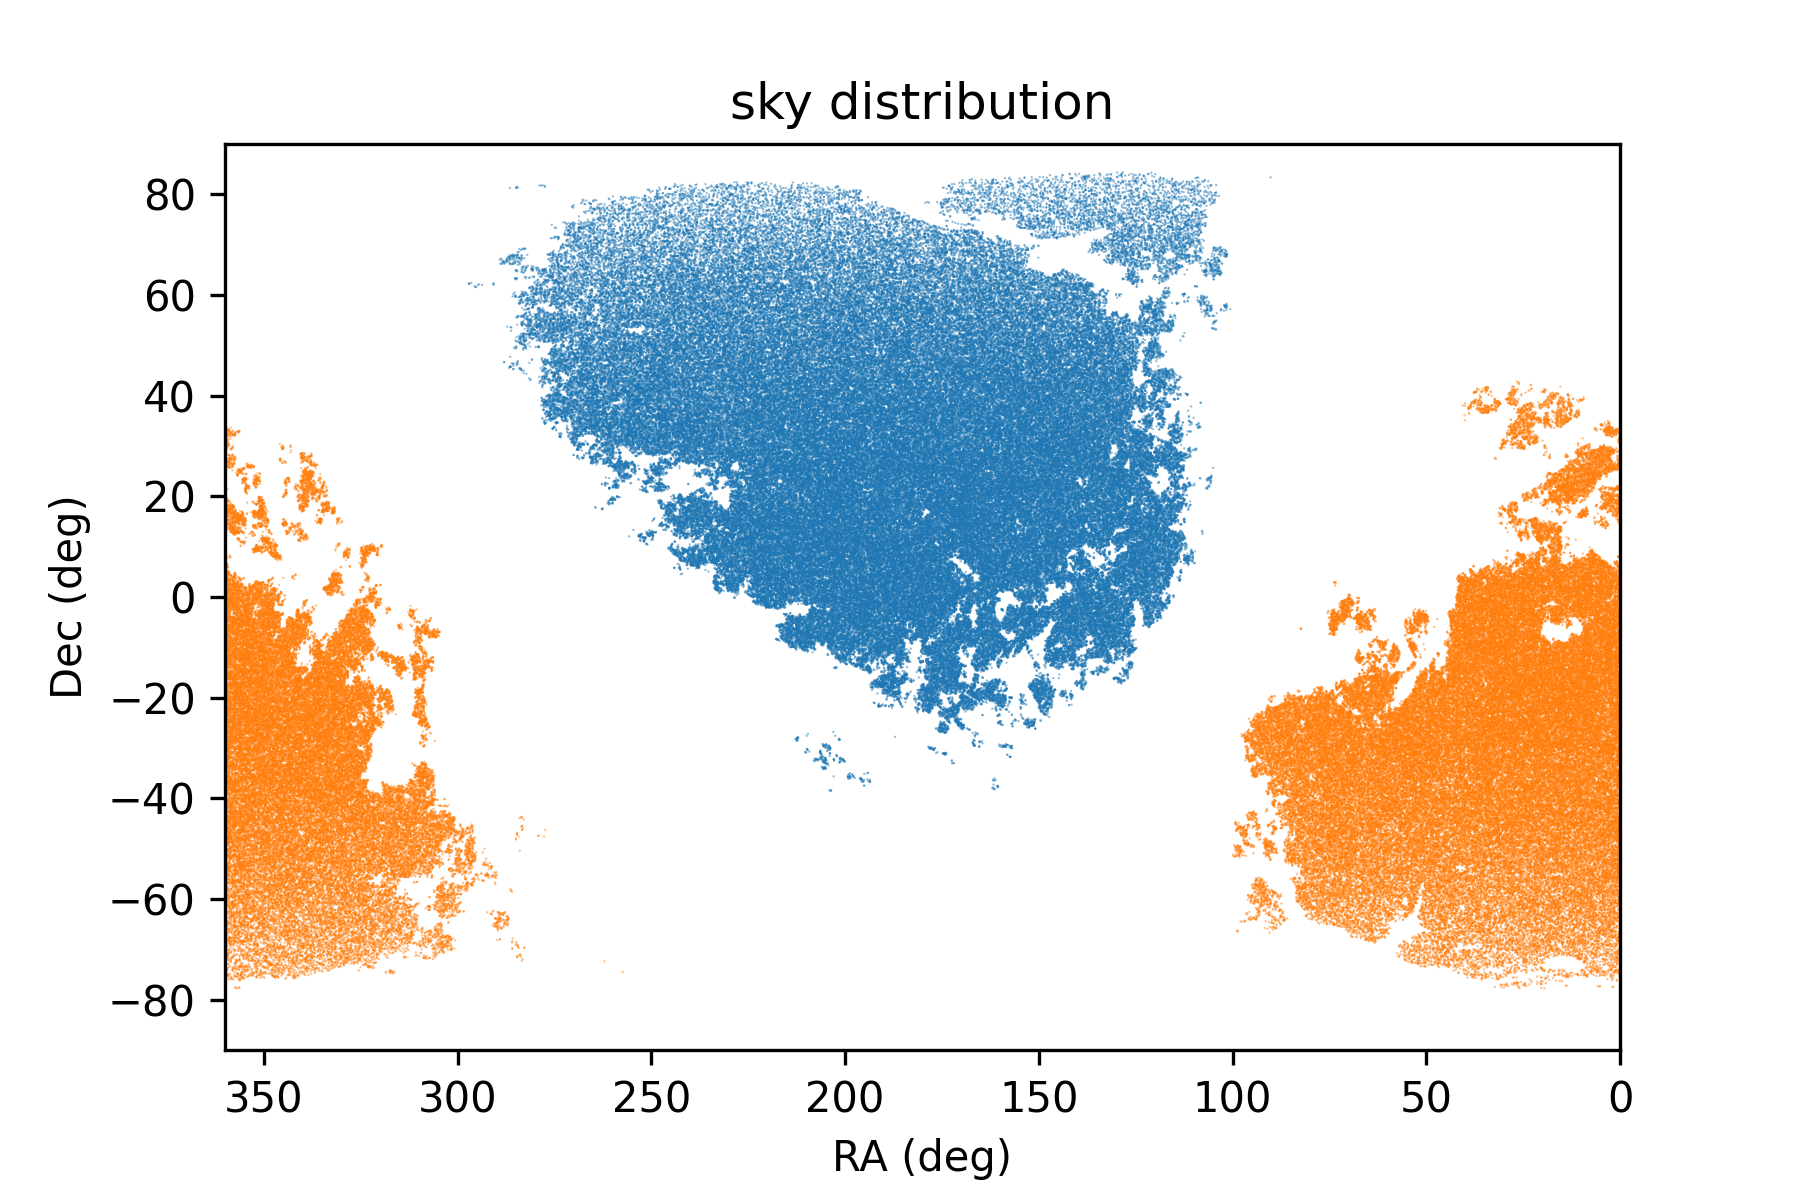
\includegraphics[width=\figurewidth]{notebooks/radec.png}
  \end{center}
    \caption{The full quasar sample plotted on the sky in Equatorial coordinates.
    The NGC subsample (and its associated random catalog) is colored blue and the SGC subsample is colored orange.\label{fig:radec}.}
  \end{mdframed}
\end{figure}

\begin{figure}[t!]
  \begin{mdframed}
  \color{captiongray}
  \begin{center}
    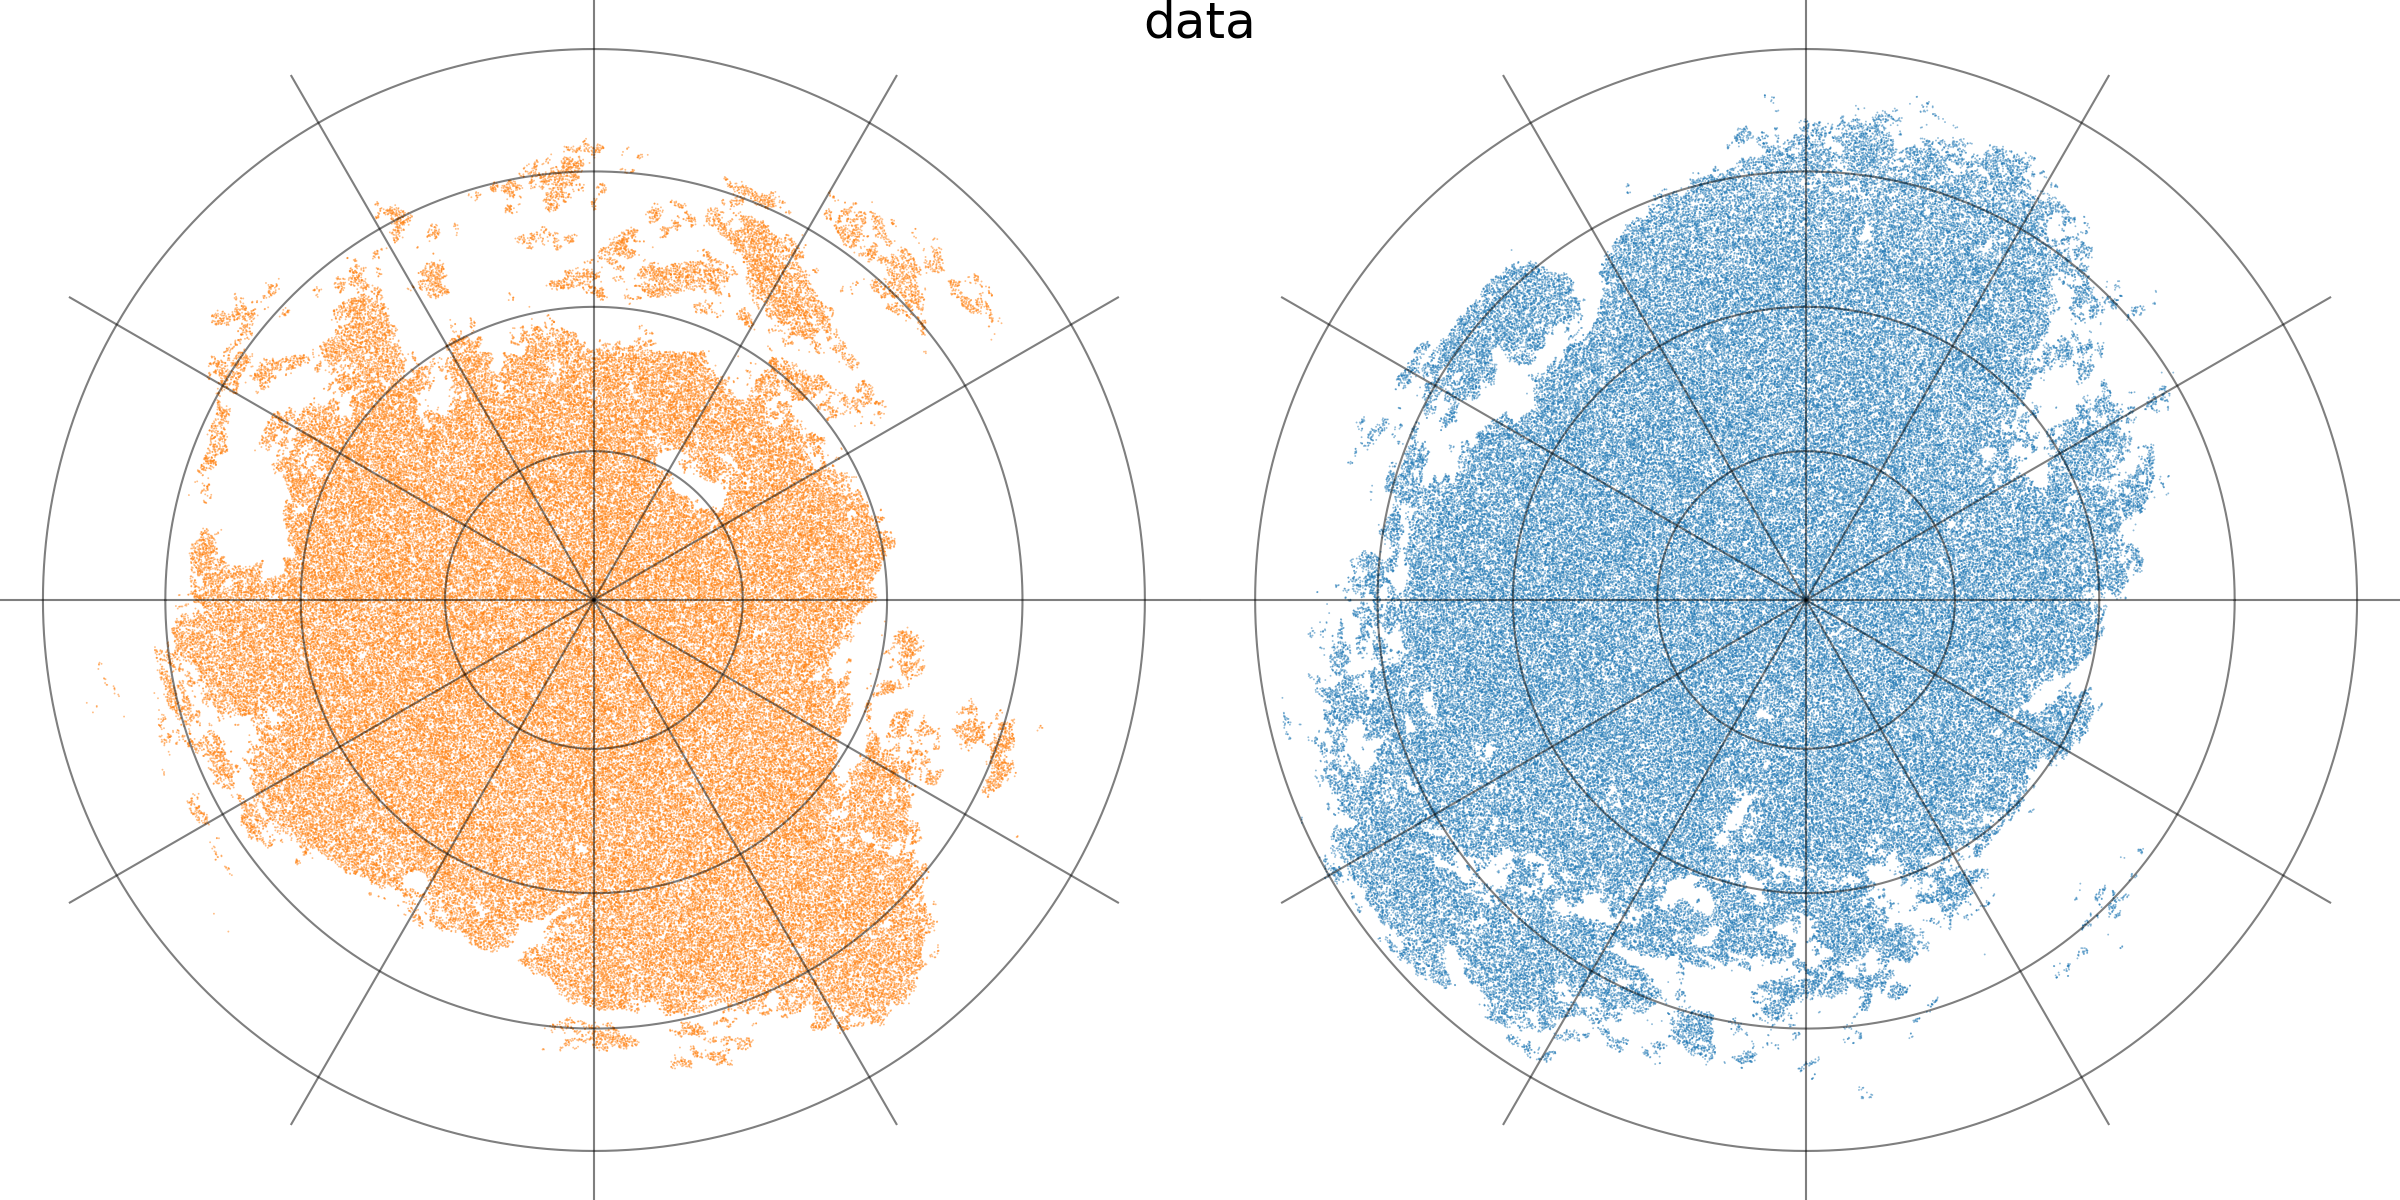
\includegraphics[width=\figurewidth]{notebooks/lb_better.png}\\
    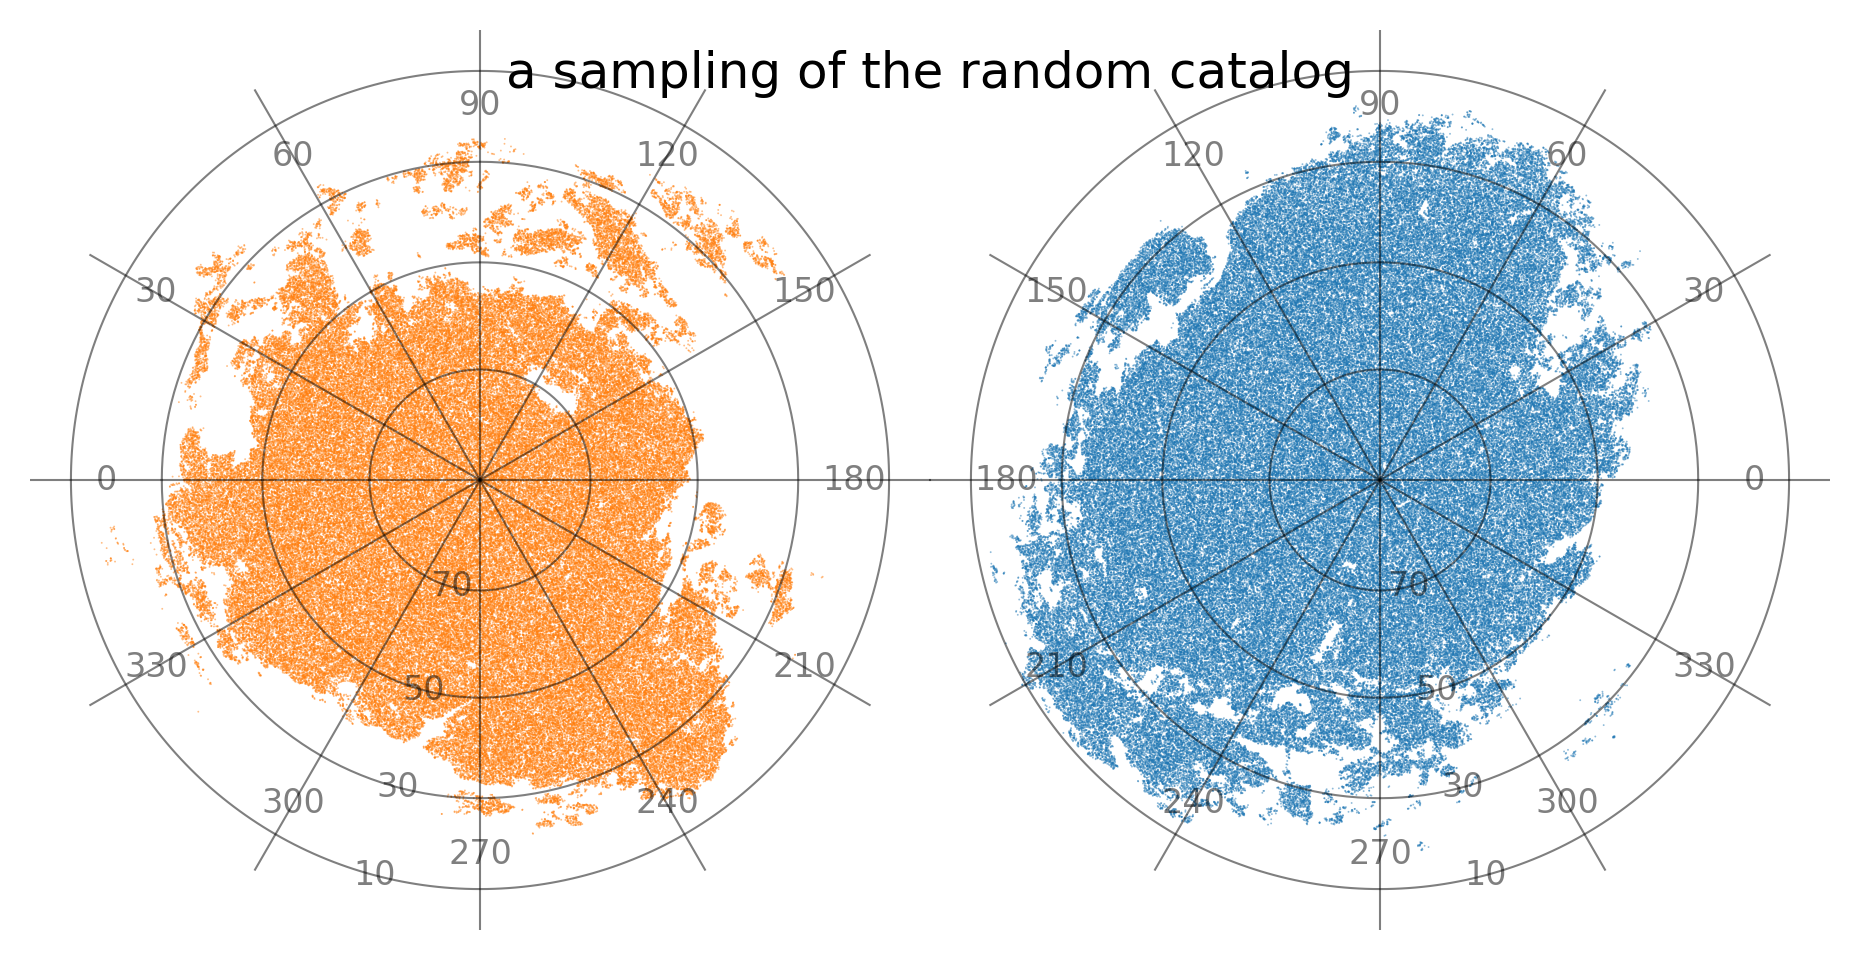
\includegraphics[width=\figurewidth]{notebooks/lb_random_better.png}
  \end{center}
    \caption{The full quasar sample and a sampling of the (much larger) random catalog, plotted on the sky in Galactic coordinates.
    The sine is taken of the Galactic latitude coordinate to make the projection equal-area.
    The NGC subsample (and its associated random catalog) is colored blue and the SGC subsample is colored orange.\label{fig:lb}.}
  \end{mdframed}
\end{figure}

\section{Method and results}

\begin{figure}[t!]
  \begin{mdframed}
  \color{captiongray}
  \begin{center}
    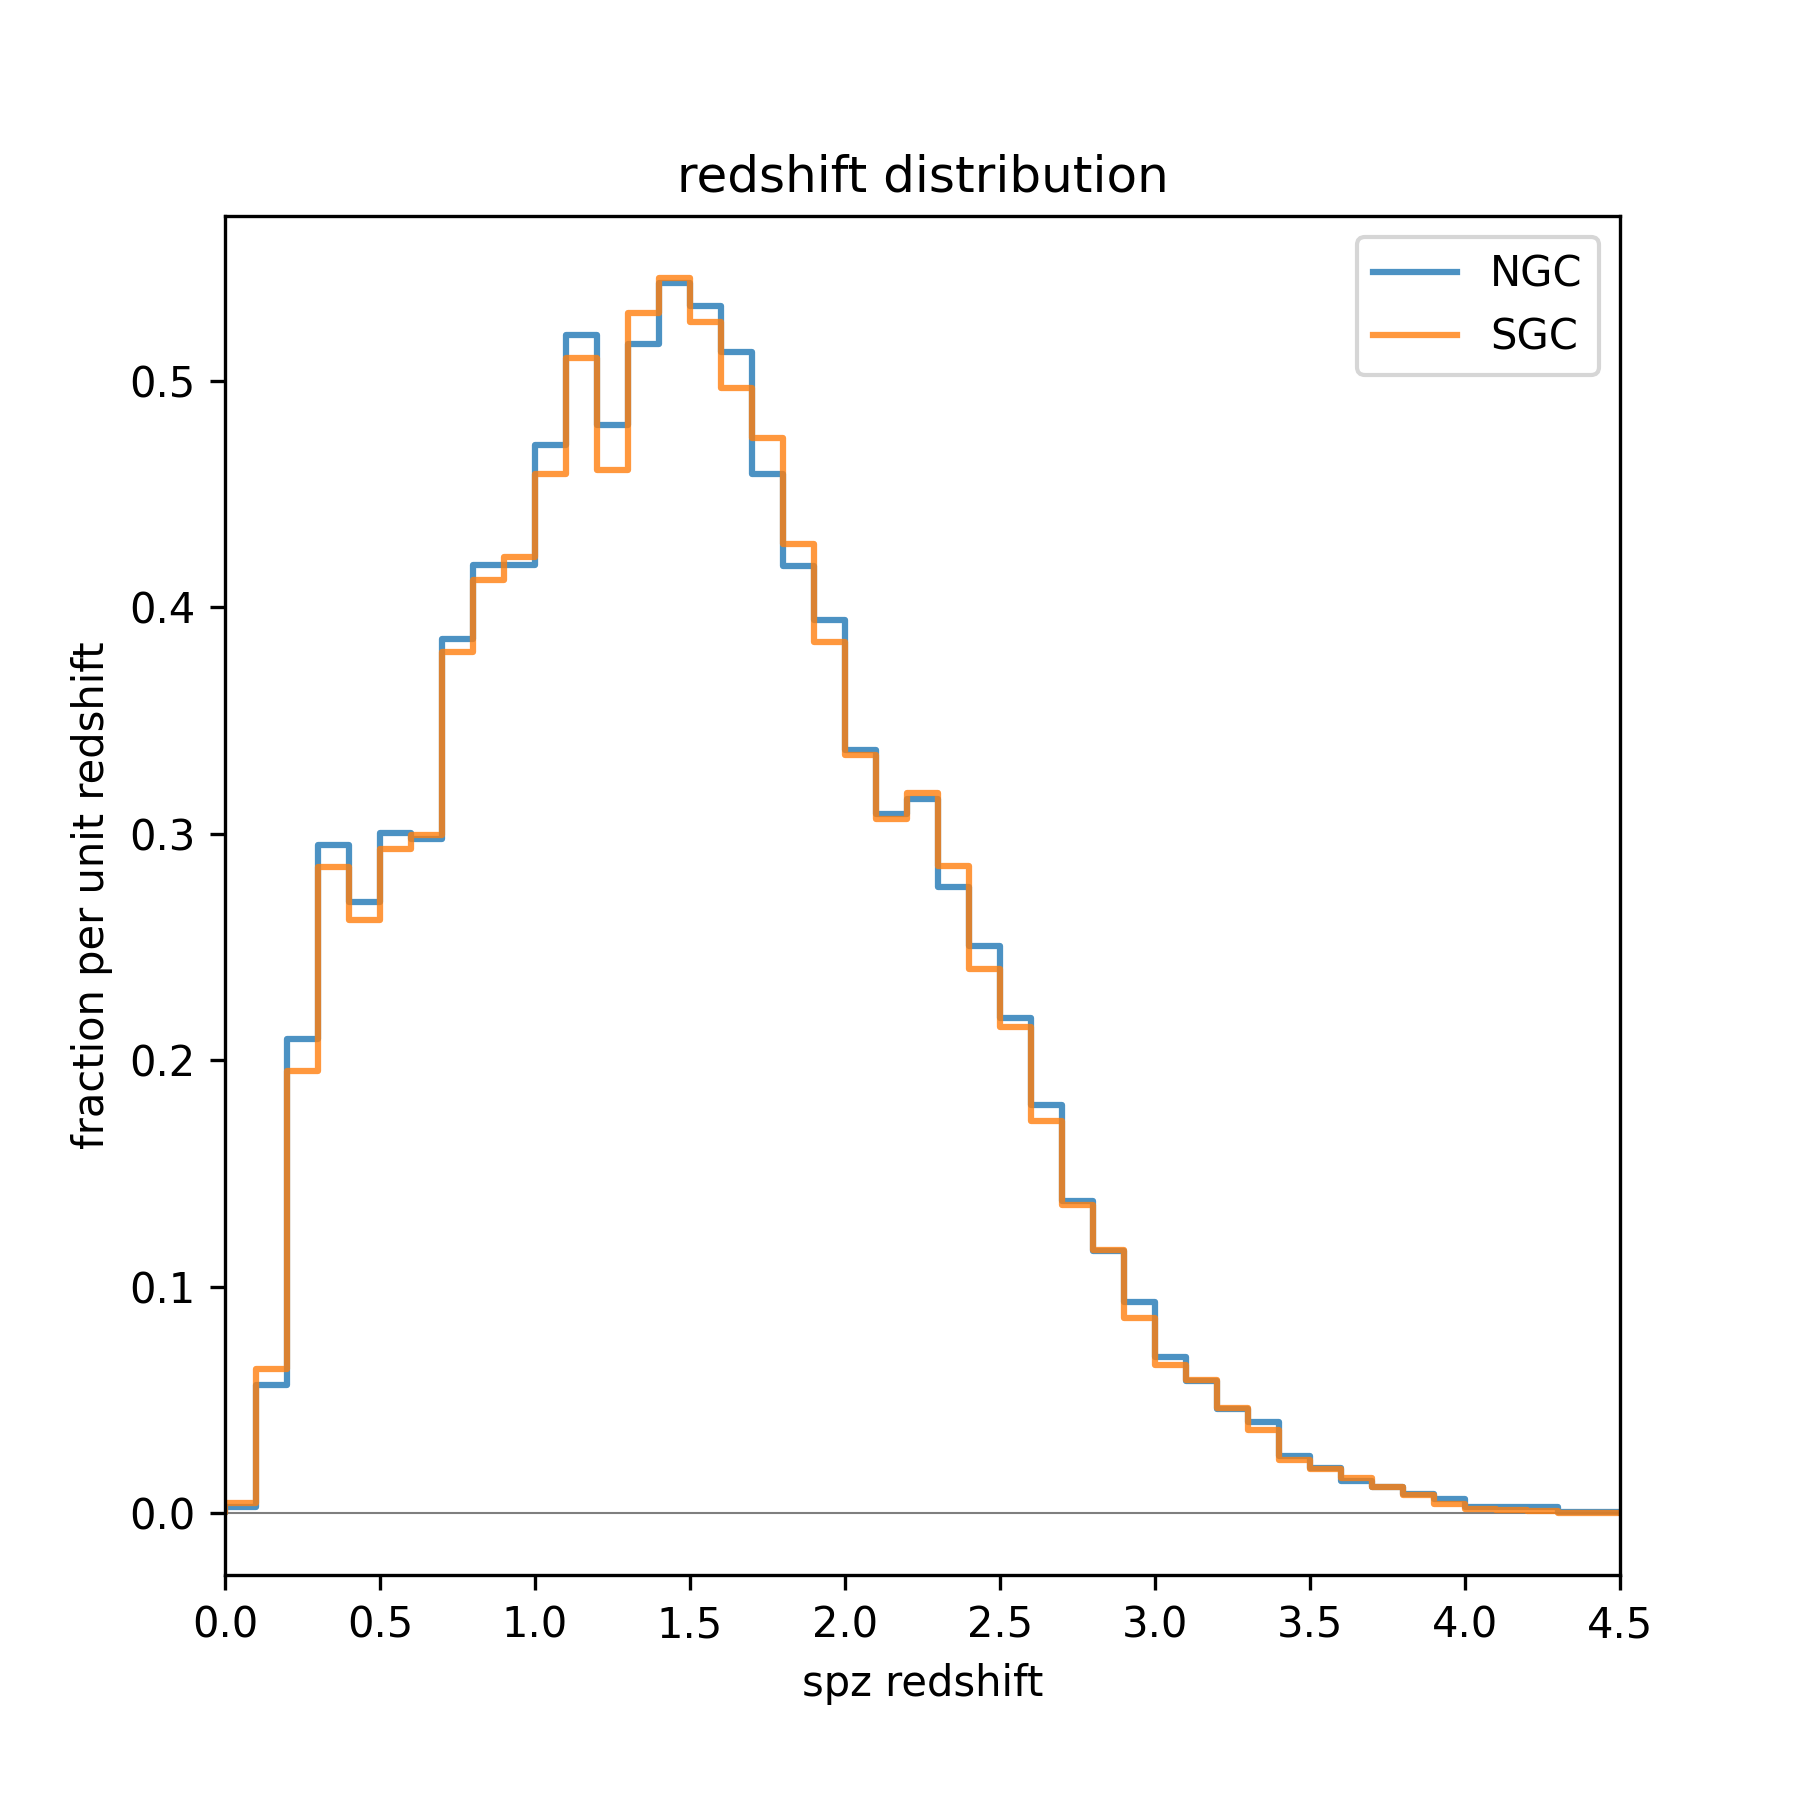
\includegraphics[width=\figurewidth]{notebooks/zhist.png}
  \end{center}
    \caption{The redshift distributions of the NGC and SGC subsamples.\label{fig:zhist}.}
  \end{mdframed}
\end{figure}

\begin{figure}[t!]
  \begin{mdframed}
  \color{captiongray}
  \begin{center}
    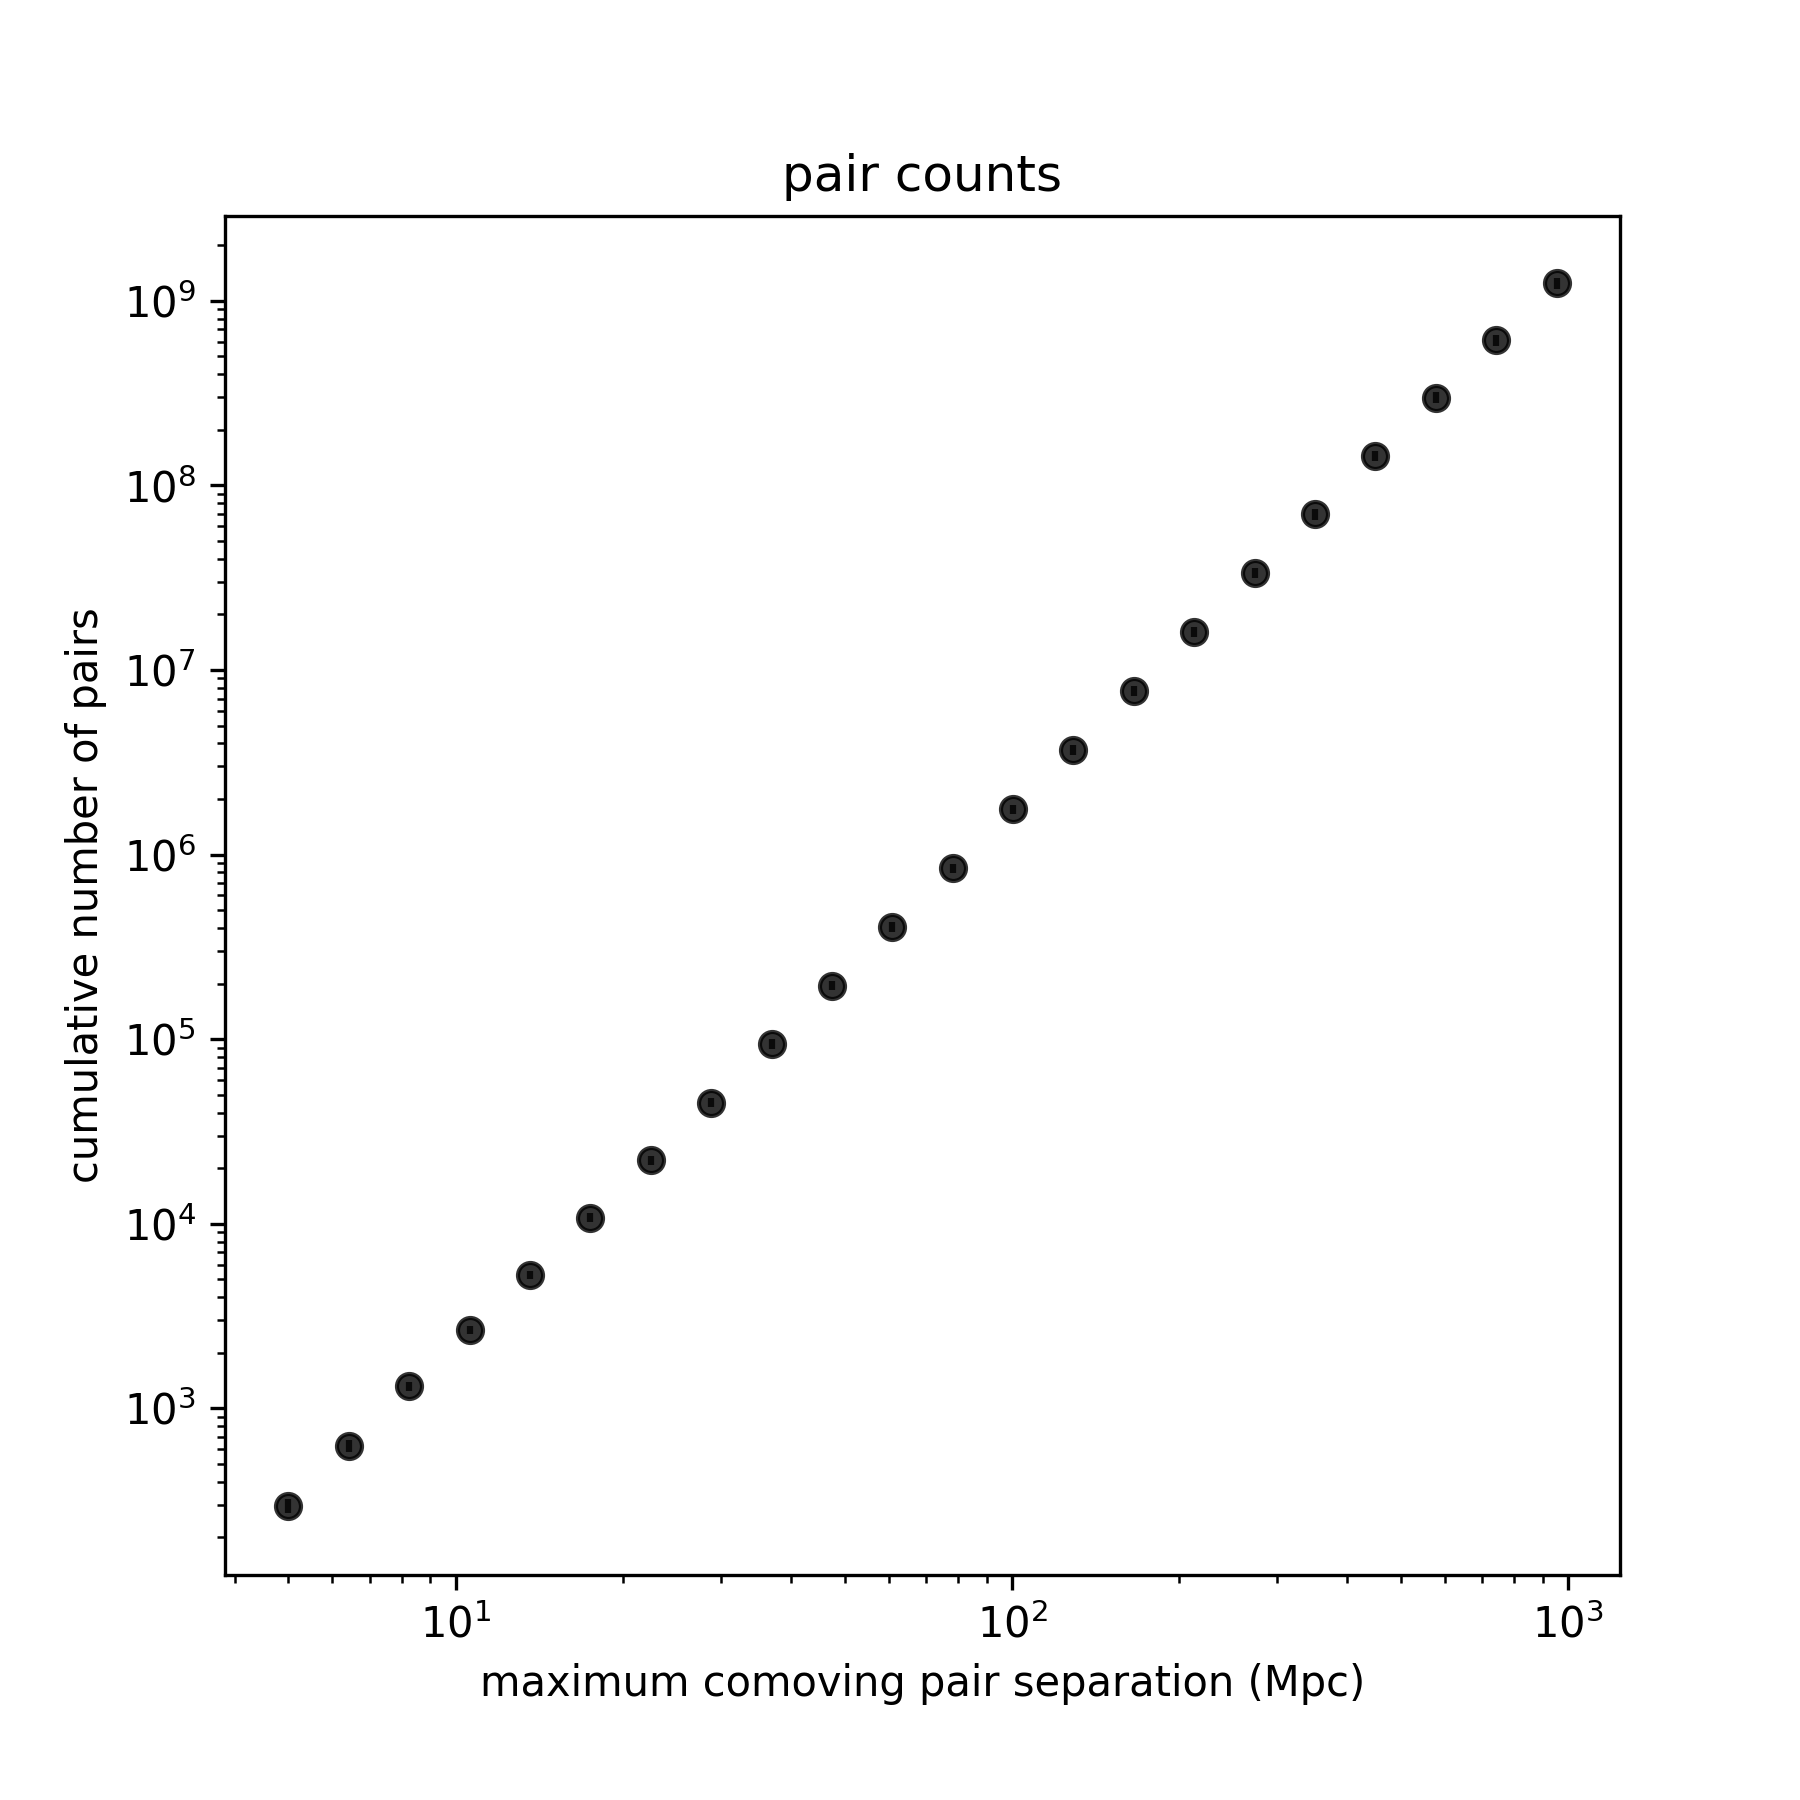
\includegraphics[width=\figurewidth]{notebooks/cumulativeDD.png}
  \end{center}
    \caption{The cumulative total number of quasar--quasar pairs as a function of separation for the NGC and SGC subsamples.
    This figure demonstrates that the fractal dimension is extremely close to 3. The small offset between the NGC and SGC comes from the differing sizes of the two regions.\label{fig:cumulative}.}
  \end{mdframed}
\end{figure}

\begin{figure}[t!]
  \begin{mdframed}
  \color{captiongray}
  \begin{center}
    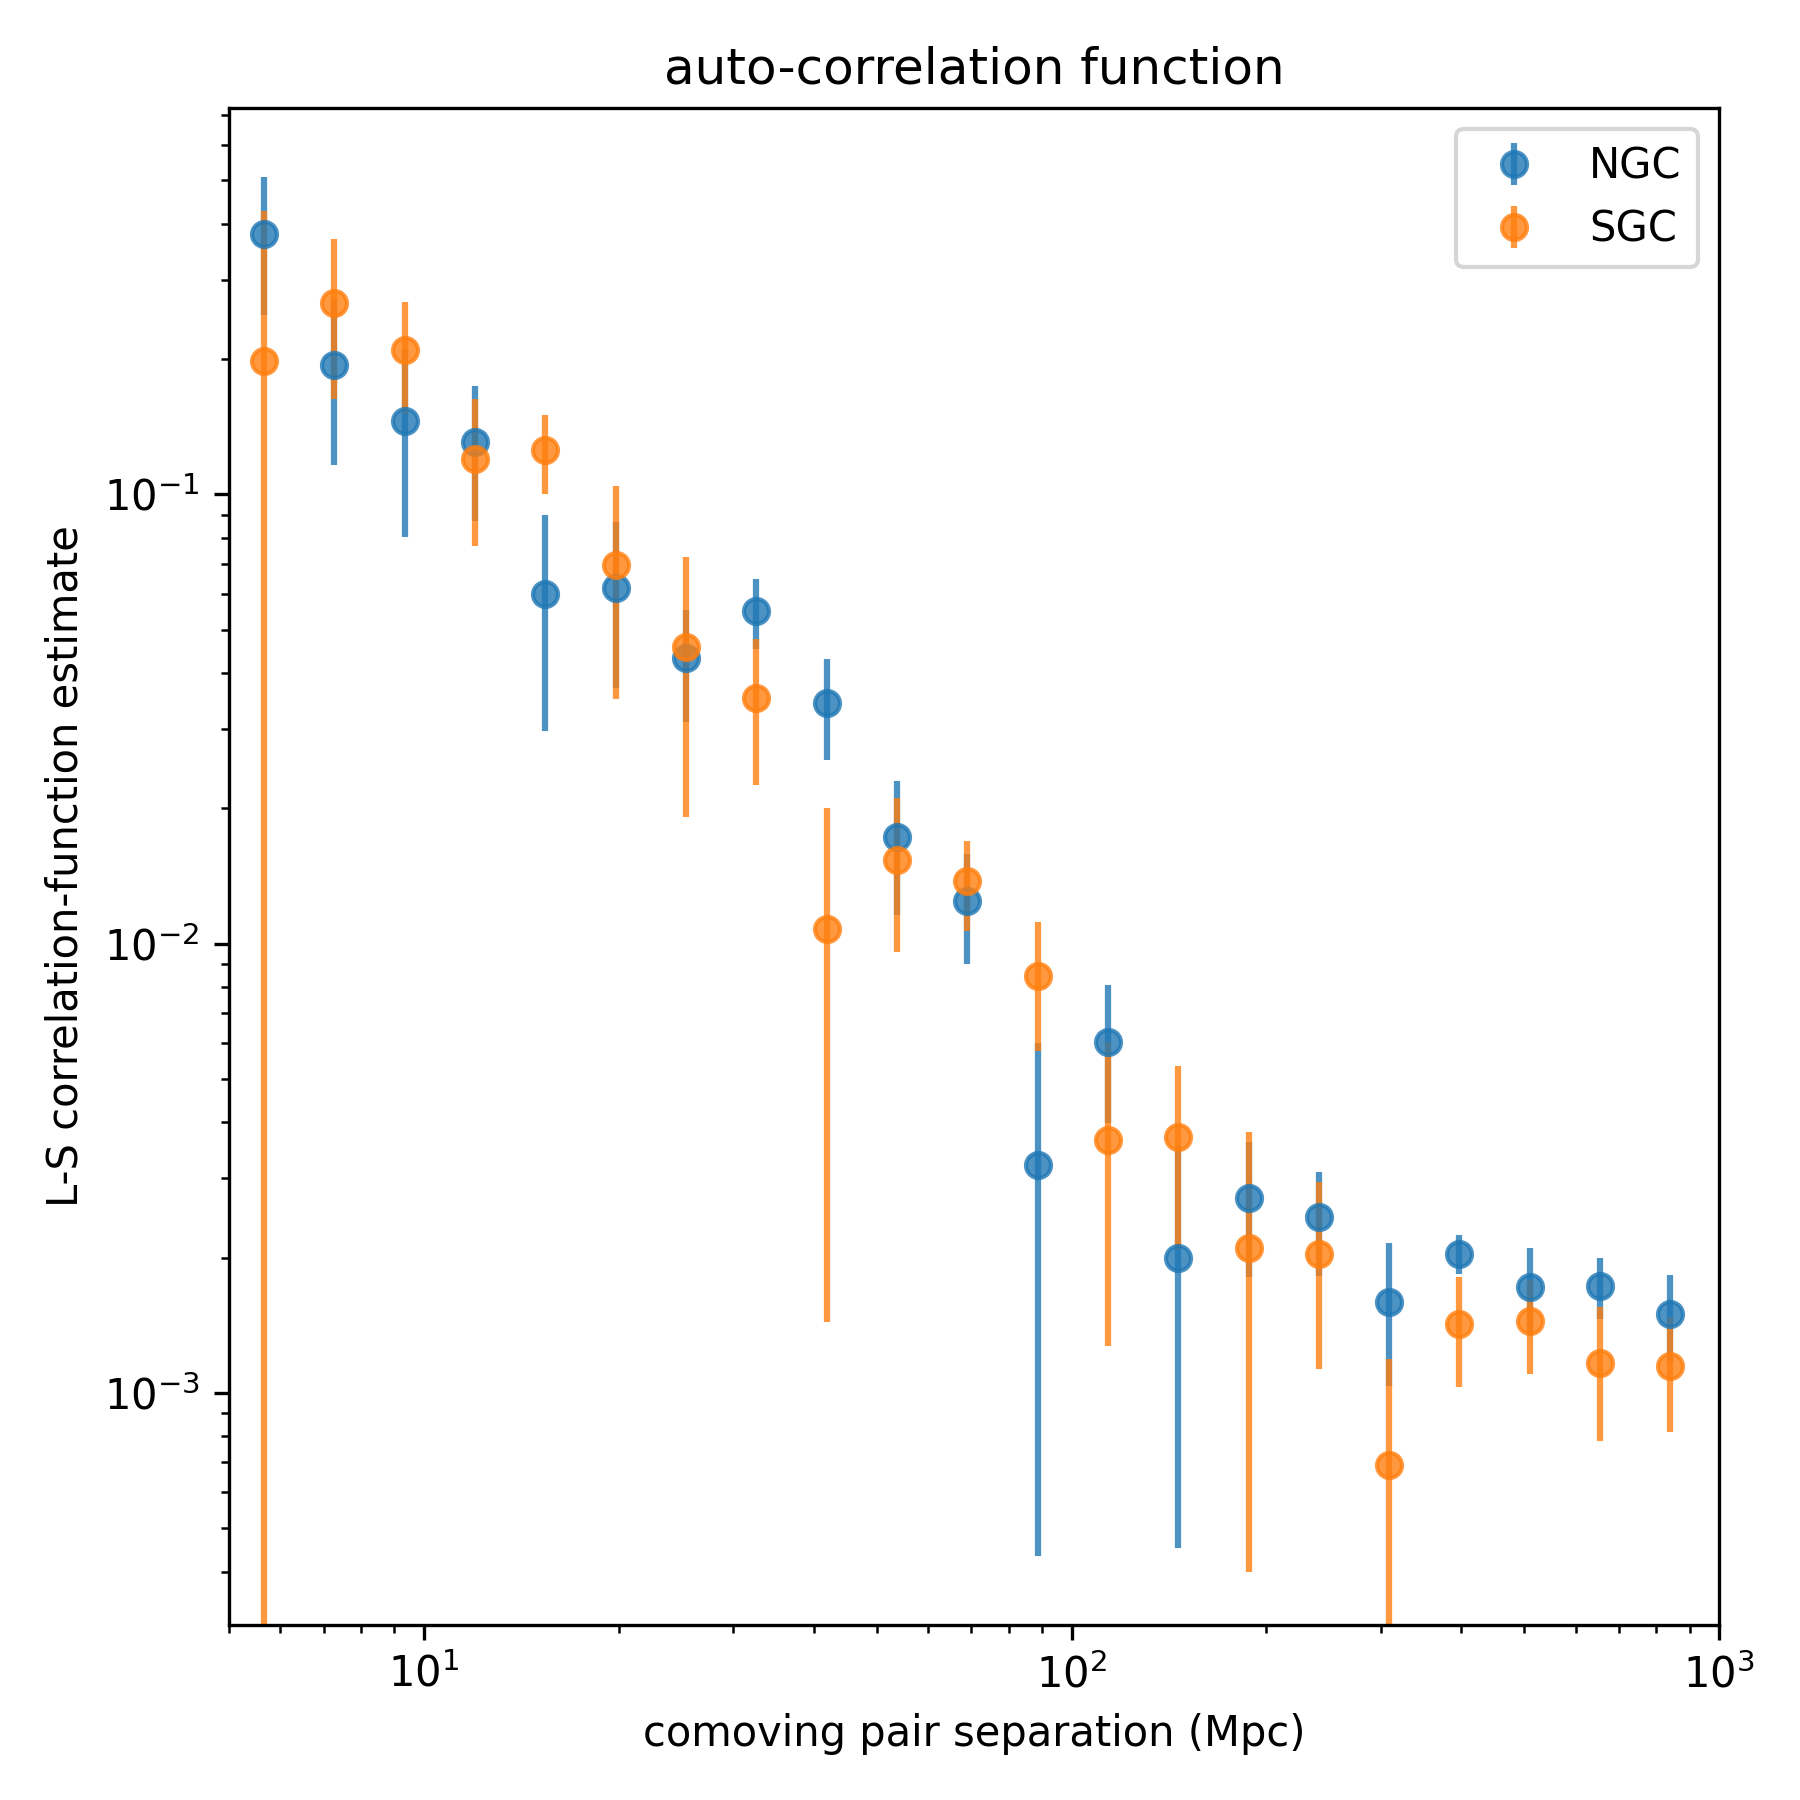
\includegraphics[width=\figurewidth]{notebooks/corrfunc.png}
  \end{center}
    \caption{The auto-correlation of the quasars as a function of separation for the NGC and SGC subsamples.
    This figure demonstrates that the clustering amplitude is similar between the North and the South.\label{fig:corrfunc}.}
  \end{mdframed}
\end{figure}

\section{Discussion}

\end{document}
